\chapter{Réseaux}
\label{chap:networks}

\section{Graphes}

Les graphes sont un outil puissant de modélisation.
Ils interviennent naturellement dans la représentation de réseaux de transport ou de télécommunication, par exemple, mais également dans la représentation de structures relationnelles abstraites.
Mathématiquement, un graphe $G$ prend la forme $G = (N,A)$ où $N$ est
un ensemble de {\sl sommets} et $A \subseteq N \times N$ un ensemble d'{\sl arcs}.
Le terme réseau est un terme générique désignant un graphe dont les sommets ou les arcs possèdent des attributs: coûts, capacités, longueurs, etc.

\subsection{Graphe orienté}

\begin{example}[Réseau de distribution]

Nous reprenons l'exemple~\ref{ex:distribution}, illustré sur la Figure~\ref{fig:net_distribution}.
Les liens entre les noeuds du graphe ne peuvent être parcourus que dans un sens précis; nous parlerons de graphe {\sl orienté}.
Les {\sl sommets} du graphe sont $A$, $B$, $C$, $D$, $E$, et le graphe posséde les {\sl arcs} $(A,B)$, $(A,C)$, $(A,D)$, $(B,C)$, $(C,E)$, $(D,E)$, $(E,D)$.
\begin{figure}[htbp]
\begin{center}
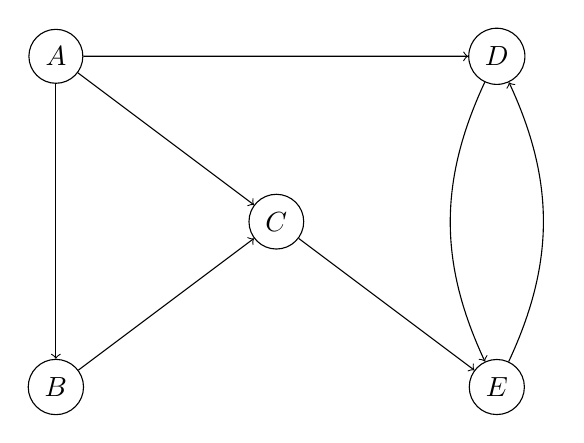
\begin{tikzpicture}[scale=0.7,->]
\node[circle,draw] (A) at (1,6) {$A$};
\node[circle,draw] (B) at (1,0) {$B$};
\node[circle,draw] (D) at (9,6) {$D$};
\node[circle,draw] (E) at (9,0) {$E$};
\node[circle,draw] (C) at (5,3) {$C$};
\path
  (A) edge (D)
  (A) edge (B)
  (A) edge (C)
  (B) edge (C)
  (C) edge (E)
;
\draw [->] (D) to [bend right=25] (E);
\draw [->] (E) to [bend right=25] (D);
\end{tikzpicture}
\caption{Réseau de distribution}
\label{fig:net_distribution}
\end{center}
\end{figure}
\end{example}

\subsection{Graphe non orienté}

\begin{example}[Parc Seervada]
\label{ex:parc_seervada}

Considérons le graphe représenté sur la Figure~\ref{fig:undirected graph}, tiré de Hillier et Lieberman~\cite{HillLieb01}, Section~9.1.
Nous avons les sommets $O$, $A$, $B$, $C$, $D$, $E$, $T$, et les {\sl arêtes}: $\lbrace O,A \rbrace$, $\lbrace O,B \rbrace$, $\lbrace O,C \rbrace$, $\lbrace A,B \rbrace$, $\lbrace A,D \rbrace$, $\lbrace B,C \rbrace$,
$\lbrace B,D \rbrace$, $\lbrace B,E \rbrace$, $\lbrace D,E \rbrace$, $\lbrace D,T \rbrace$, $\lbrace E,T \rbrace$.
Le nombre sur chaque arête représente la distance entre les deux sommets reliés par cette arête
\begin{figure}[htbp]
\begin{center}
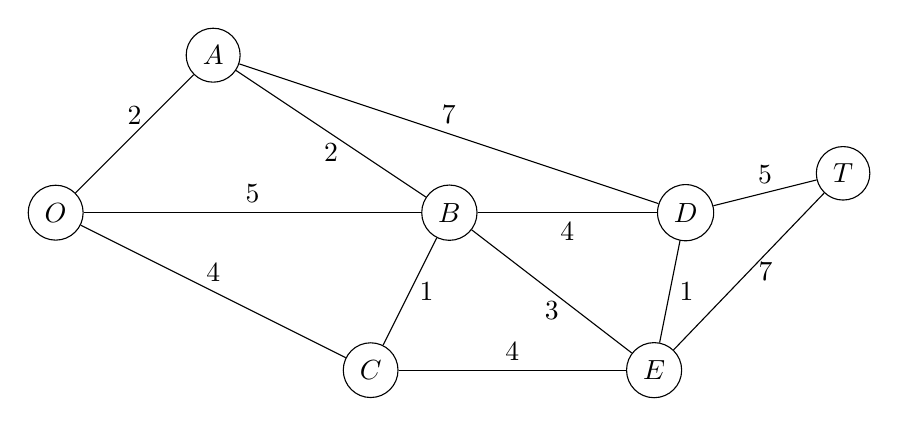
\begin{tikzpicture}
\node[circle,draw] (A) at (2,4) {$A$};
\node[circle,draw] (O) at (0,2) {$O$};
\node[circle,draw] (C) at (4,0) {$C$};
\node[circle,draw] (B) at (5,2) {$B$};
\node[circle,draw] (D) at (8,2) {$D$};
\node[circle,draw] (E) at (7.6,0) {$E$};
\node[circle,draw] (T) at (10,2.5) {$T$};
\path
  (O) edge node [above,midway] {2} (A)
  (O) edge node [above,midway] {5} (B)
  (O) edge node [above,midway] {4} (C)
  (A) edge node [below,midway] {2} (B)
  (A) edge node [above,midway] {7} (D)
  (B) edge node [below,midway] {4} (D)
  (B) edge node [below,midway] {3} (E)
  (E) edge node [right,midway] {1} (D)
  (D) edge node [above,midway] {5} (T)
  (C) edge node [right,midway] {1} (B)
  (E) edge node [right,midway] {7} (T)
  (C) edge node [above,midway] {4} (E)
;
\end{tikzpicture}
\caption{Graphe non orienté}
\label{fig:undirected graph}
\end{center}

\end{figure}
 
\end{example}

\subsection{Transformations}

Un graphe orienté dérivé d'un graphe non orienté en introduisant deux arcs pour chaque arête, un dans chaque direction.
A l'inverse, nous qualifierons de graphe sous-jacent à un graphe orienté le graphe obtenu en enlevant l'orientation des arcs.
Si $G$ est un graphe orienté, le graphe dérivé du graphe sous-jacent à $G$ n'est pas $G$.

\subsection{Chemins et circuits}

Un {\sl chemin} [chaîne] est suite d'arcs [d'arêtes] distinct[e]s reliant deux sommets.
Il est non orienté s'il est constitué d'une suite d'arcs distincts qui relient deux sommets, sans considération de l'orientation des arcs.
En d'autres mots, un chemin non orienté est une chaîne dans le graphe sous-jacent.
Un {\sl circuit} [cycle] est un chemin [chaîne] qui commence et finit au même sommet.
Le circuit est non orienté s'il s'agit d'un cycle dans le graphe sous-jacent.

\begin{example}[Réseau de distribution]

Reprenons l'exemple du réseau de distribution, illustré sur la Figure~\ref{fig:net_distribution_2}.
$A \rightarrow C \rightarrow E \rightarrow D$ décrit un chemin, et en ignorant l'orientation des arcs, nous décrivons également un chemin non orienté.
$A \rightarrow D \rightarrow E \rightarrow C \rightarrow B$ est chemin non orienté, mais pas un chemin.
$D \rightarrow E \rightarrow D$ est circuit, et en omettant l'orientation des arcs, un circuit non orienté.
$A \rightarrow B \rightarrow C \rightarrow A$ est un circuit non orienté (mais pas un circuit).
\begin{figure}[htbp]
\begin{center}
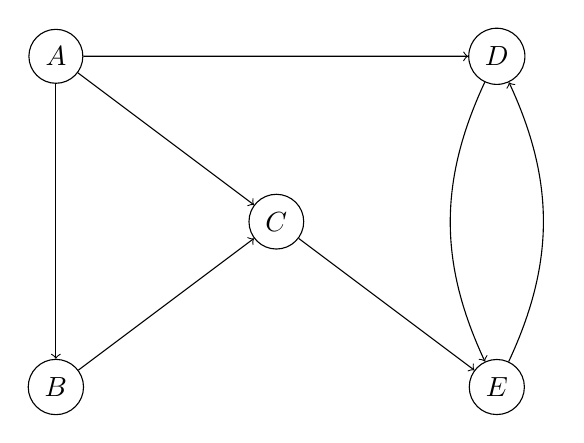
\begin{tikzpicture}[scale=0.7,->]
\node[circle,draw] (A) at (1,6) {$A$};
\node[circle,draw] (B) at (1,0) {$B$};
\node[circle,draw] (D) at (9,6) {$D$};
\node[circle,draw] (E) at (9,0) {$E$};
\node[circle,draw] (C) at (5,3) {$C$};
\path
  (A) edge (D)
  (A) edge (B)
  (A) edge (C)
  (B) edge (C)
  (C) edge (E)
;
\draw [->] (D) to [bend right=25] (E);
\draw [->] (E) to [bend right=25] (D);
\end{tikzpicture}
\caption{Réseau de distribution}
\label{fig:net_distribution_2}
\end{center}
\end{figure}
\end{example}

\subsection{Connexité}

Deux sommets sont connexes s'il existe au moins un chemin non orienté les reliant.
Un graphe est connexe si toute paire de sommets est connexe.
Le plus petit graphe connexe à $n$ sommets possède $n-1$ arêtes; il est appelé un {\sl arbre}.
Une définition alternative consiste à dire qu'un arbre est un graphe connexe sans cycle.
Un arbre partiel est un arbre obtenu à partir d'un graphe connexe en incluant tous les sommets.

\begin{example}
Retournons sur l'exemple~\ref{ex:parc_seervada}.
Le graphe ci-dessous n'est pas un arbre partiel, comme il n'est pas connexe.

\begin{center}
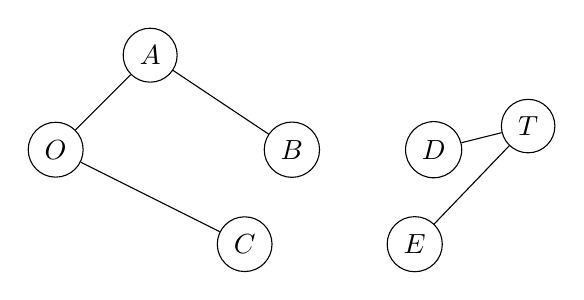
\begin{tikzpicture}[scale=0.6]
\node[circle,draw] (A) at (2,4) {$A$};
\node[circle,draw] (O) at (0,2) {$O$};
\node[circle,draw] (C) at (4,0) {$C$};
\node[circle,draw] (B) at (5,2) {$B$};
\node[circle,draw] (D) at (8,2) {$D$};
\node[circle,draw] (E) at (7.6,0) {$E$};
\node[circle,draw] (T) at (10,2.5) {$T$};
\path
  (O) edge (A)
  (O) edge (C)
  (A) edge (B)
  (D) edge (T)
  (E) edge (T)
;
\end{tikzpicture}
\end{center}

Le graphe ci-dessous est connexe, mais présente des cycles.
Par conséquent, il ne s'agit pas d'un arbre.
\begin{center}
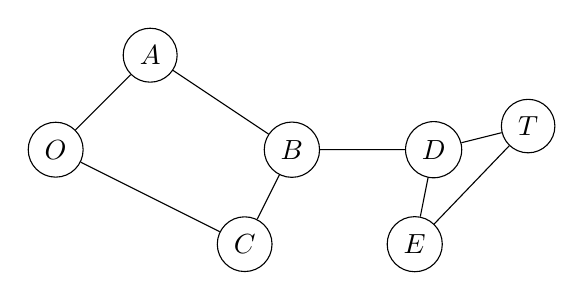
\begin{tikzpicture}[scale=0.6]
\node[circle,draw] (A) at (2,4) {$A$};
\node[circle,draw] (O) at (0,2) {$O$};
\node[circle,draw] (C) at (4,0) {$C$};
\node[circle,draw] (B) at (5,2) {$B$};
\node[circle,draw] (D) at (8,2) {$D$};
\node[circle,draw] (E) at (7.6,0) {$E$};
\node[circle,draw] (T) at (10,2.5) {$T$};
\path
  (O) edge (A)
  (O) edge (C)
  (A) edge (B)
  (B) edge (D)
  (E) edge (D)
  (D) edge (T)
  (C) edge (B)
  (E) edge (T)
;
\end{tikzpicture}
\end{center}

Le graphe ci-dessous est un arbre partiel.
\begin{center}
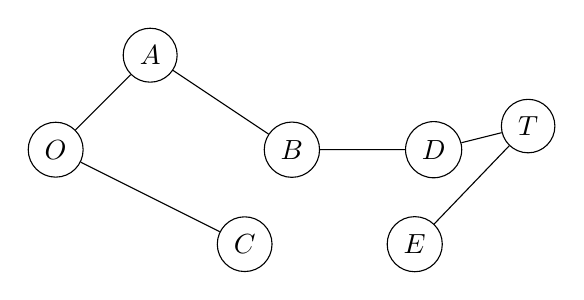
\begin{tikzpicture}[scale=0.6]
\node[circle,draw] (A) at (2,4) {$A$};
\node[circle,draw] (O) at (0,2) {$O$};
\node[circle,draw] (C) at (4,0) {$C$};
\node[circle,draw] (B) at (5,2) {$B$};
\node[circle,draw] (D) at (8,2) {$D$};
\node[circle,draw] (E) at (7.6,0) {$E$};
\node[circle,draw] (T) at (10,2.5) {$T$};
\path
  (O) edge (A)
  (O) edge (C)
  (A) edge (B)
  (B) edge (D)
  (D) edge (T)
  (E) edge (T)
;
\end{tikzpicture}
\end{center}
\end{example}

\section{Problème du chemin le plus court - algorithmes de corrections d'étiquettes}

Considérons un graphe non orienté et connexe, sur lequel deux sommets ont un rôle particulier:
\begin{itemize}
 \item
  source (ou origine): $O$;
 \item
  puits (ou destination): $T$.
\end{itemize}
A chaque arête $\lbrace i,j \rbrace$, nous associons une distance $c_{ij} \geq 0$.
Nous cherchons le chemin non orienté (ou chaîne) le plus court reliant $O$ à $T$.
Par chemin le plus court, nous désignons celui dont la distance totale (somme des distances des arêtes du chemin) est minimale parmi tous les chemins de $O$ à $T$.
Afin de procéder, nous affectons à chaque noeud du graphe une étiquette, représentant la meilleure distance  connue à un moment donné, de l'origine à ce noeud.

\subsection{Algorithme de Dijkstra}

Il s'agit d'une méthode itérative
A chaque itération, nous choisissons le sommet $j$ le plus près de $O$ et nous fixons $d(j)$, la variable calculant la distance entre $0$ et $j$
(le sommet $j$ est dit marqué).
Au départ, seul $O$ est marqué et $d(O) = 0$.
Le sommet le plus près est choisi parmi les sommets non marqués reliés à au moins un sommet marqué.
Le sommet choisi $j$ est celui qui atteint
\[
\min_{\mbox{sommets $k$ non marqués}} \left\lbrace \min_{\mbox{sommets $i$ marqués}} d(i) + c_{ik} \right\rbrace.
\]
$d(j)$ est fixée à cette valeur.
Nous nous arrêtons lorsque $T$ est marqué si nous cherchons à connaître le chemin allant de $O$ à $T$ spécifiquement, ou sinon jusqu'à avoir marqué tous les sommets.
Par la suite, nous supposerons dans la description que nous voulons marquer tous les sommets.
Plus spécifiquement, nous avons l'algorithme ci-dessous.
L'algorithme de Dijkstra s'applique aussi sur un graphe orienté.

\begin{algo}{Algorithme de Dijkstra}

Soient $G = (N,A)$ un graphe connexe, de longueur d'arêtes non-négative (la longueur des arêtes est donnée par une fonction $\ell: A \rightarrow \RR^+$), une source $O \in N$.
Désignons par $S$ l'ensemble des sommets marqués.
\begin{enumerate}
\item Initialisation. Pour tout $u \in N$, faire
\begin{itemize}
\item
dist($u$) := $\infty$;
\item
pred(u) := NULL.
\end{itemize}
où pred($u$) indique le prédécesseur de $u$ sur le plus court chemin de $O$ à $u$.
Le noeud origine prend un rôle particulier, et comme il est évident que le plus court chemin de $O$ à $O$ a une longueur nulle, nous posons dist($O$) = 0.
Comme à ce stade, aucun noeud n'a encore été marqué, nous posons $S = \emptyset$.
\item
Tant que $S \ne N$, prenons $u$ tel que
\[
\mbox{dist}(u) \leq \mbox{dist}(v),\ \forall v \in N \backslash S.
\]
Posons $S := S \cup \lbrace u \rbrace$, et, pour tout arc $(u,v)$ existant, si
\[
\mbox{dist}(v) < \mbox{dist}(u) + \ell(u,v),
\]
posons
\begin{align*}
& \mbox{dist}(v) := \mbox{dist}(u) + \ell(u,v),\\
& \mbox{pred}(v) = u.
\end{align*}
\end{enumerate}
\end{algo}
Il est possible de montrer qu'une fois un noeud $u$ marqué, dist($u$) donne la longueur du plus court chemin de $O$ à $u$.

\begin{example}
L'application de l'algorithme de Dijkstra pour l'exemple~\ref{ex:parc_seervada}, repris à la Figure~\ref{fig:dijkstra}, donne
la série d'itérations résumée dans la Table~\ref{tab:dijkstra}.
\begin{figure}[htbp]
\begin{center}
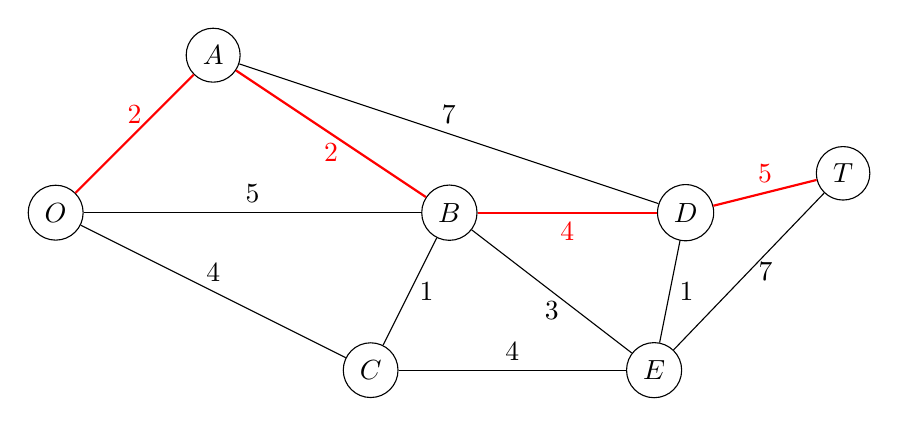
\begin{tikzpicture}
\node[circle,draw] (A) at (2,4) {$A$};
\node[circle,draw] (O) at (0,2) {$O$};
\node[circle,draw] (C) at (4,0) {$C$};
\node[circle,draw] (B) at (5,2) {$B$};
\node[circle,draw] (D) at (8,2) {$D$};
\node[circle,draw] (E) at (7.6,0) {$E$};
\node[circle,draw] (T) at (10,2.5) {$T$};
\path
  (O) edge[color=red,thick] node [above,midway] {2} (A)
  (O) edge node [above,midway] {5} (B)
  (O) edge node [above,midway] {4} (C)
  (A) edge[color=red,thick] node [below,midway] {2} (B)
  (A) edge node [above,midway] {7} (D)
  (B) edge[color=red,thick] node [below,midway] {4} (D)
  (B) edge node [below,midway] {3} (E)
  (E) edge node [right,midway] {1} (D)
  (D) edge[color=red,thick] node [above,midway] {5} (T)
  (C) edge node [right,midway] {1} (B)
  (E) edge node [right,midway] {7} (T)
  (C) edge node [above,midway] {4} (E)
;
\end{tikzpicture}
\caption{Plus court chemin}
\label{fig:dijkstra}
\end{center}
\end{figure}

\begin{table}[htbp]
\begin{center}
\begin{tabular}{|c|c|c|c|c|c|c|}
\hline
Itération & Sommet & $S$ & $N\backslash S$ & Voisins & Distance & Prédécesseur \\
& marqué & & & non marqués & & \\
\hline
0 & - & $\emptyset$ & $N$ & - & - & - \\
\hline
1 & $O$ & $\lbrace O \rbrace$ & $\lbrace A, B, C, D, E, T \rbrace$ &
$A$ & 2 & $O$ \\
& & & & $B$ & 5 & $O$ \\
& & & & $C$ & 4 & $O$ \\
\hline
2 & $A$ & $\lbrace O, A \rbrace$ & $\lbrace B, C, D, E, T \rbrace$ &
$B$ & 4 & $A$ \\
& & & & $D$ & 9 & $A$ \\
\hline
3 & $B$ & $\lbrace O, A, B \rbrace$ & $\lbrace C, D, E, T \rbrace$ &
$D$ & 8 & $B$ \\
& & & & $C$ & 4 & $O$ \\
& & & & $E$ & 7 & $B$ \\
\hline
4 & $C$ & $\lbrace O, A, B, C \rbrace$ & $\lbrace D, E, T \rbrace$ &
$E$ & 7 & $B$ \\
\hline
5 & $E$ & $\lbrace O, A, B, C, E \rbrace$ & $\lbrace D, T \rbrace$ &
$D$ & 8 & $B$ \\
& & & & $T$ & 14 & $E$ \\
\hline
6 & $D$ & $\lbrace O, A, B, C, D, E \rbrace$ & $\lbrace T \rbrace$ &
$T$ & 13 & $D$ \\
\hline
7 & $T$ & $N$ & $\emptyset$ & - & - & - \\
\hline
\end{tabular}
\caption{Exécution de l'algorithme de Dijkstra}
\label{tab:dijkstra}
\end{center}
 
\end{table}

\end{example}

Il est également possible de trouver les chemins les plus courts entre la source
et tous les autres sommets (il suffit de regarder la valeur de $d(i)$ en chaque sommet $i$).
Nous pouvons également trouver les chemins les plus courts entre toutes les paires de sommets, avec $n$ applications de l'algorithme de Dijkstra (mais il est possible de faire mieux).
Si certaines distances sont négatives, l'algorithme de Dijkstra ne s'applique cependant pas.


\section{Flot dans un réseau}

\subsection{Réseau}

Un {\sl réseau} est un graphe orienté ayant
\begin{itemize}
 \item 
 des capacités sur les arcs;
 \item
 des sommets d'offre (ou sources);
 \item
 des sommets de demande (ou puits);
 \item
 des sommets de transfert.
\end{itemize}
Le {\sl flot} dans un réseau est le nombre d'unités circulant sur les arcs du réseau de façon à respecter les capacités et les contraintes de conservation de flot.
En chaque sommet, le flot sortant moins le flot entrant vaut
\begin{itemize}
 \item 
 l'offre (si le sommet est une source);
 \item
 la demande (si le sommet est un puits);
 \item
 0 (en un sommet de transfert).
\end{itemize}
Soit $A$ est l'ensemble des arcs du réseau.
En dénotant par $x_{ij}$ la quantité de flot qui passe sur l'arc $(i,j) \in A$, nous avons
\[
\sum_{(i,j) \in A^+(i)} x_{ij} - \sum_{(i,j) \in A^-(i) }x_{ji} = b_i,\quad i, j \in N
\]
où
\begin{itemize}
 \item 
 $b_i = 0$ (transfert), offre (source), -demande (puits);
 \item
 $N$ désigne l'ensemble des sommets;
 \item
 $A^+(i)$ est l'ensemble des arcs sortants du sommet $i$;
 \item
 $A^-(i)$ désigne l'ensemble des arcs entrants au sommet $i$;
\end{itemize}
avec $0 \leq x_{ij} \leq u_{ij}$.

\subsection{Modèle de flot}

Le chemin le plus court peut être vu comme le flot dans un réseau, lequel est le graphe orienté dérivé.
On enlève les arcs entrant à $O$ et les arcs émanant de $T$.
$O$ est la seule source, avec une offre égale à 1.
$T$ est le seul puits, avec une demande valant 1.
Le flot sur chaque arc $(i,j)$ est soit 1, si l'arc appartient au chemin le plus court, soit 0, sinon.

\subsection{Algorithme de Bellman-Ford}

La déficience majeure de l'algorithme de Dijkstra est qu'en présence d'arcs (arêtes) de poids négatif, ajouter un arc à un chemin peut faire décroître la longueur de ce chemin, de sorte que lors du marquage d'un noeud $u$, dist($u$) ne correspond plus nécessairement à la longueur du plus court chemin de $O$ à $u$.
En particulier, si considérons le plus court chemin
\[
O \rightarrow v_1 \rightarrow v_2 \rightarrow \ldots \rightarrow v_k
\]
de $O$ à $v_k$, alors il n'est plus vrai que
\[
d(O,v_i) \leq d(O,v_k) \ \forall \ i < k.
\]
Il est pourtant fréquent d'avoir des poids négatifs sur certains arcs.
L'algorithme de Bellman-Ford permet de traiter de tels cas, pour autant qu'il n'y ait pas de cycles de longueur négative, c'est-à-dire un cycle dont les sommes des poids des arêtes est strictement négatif.
En effet, s'il est possible d'atteindre de $O$ un cycle $C$ de longueur négative, et qu'il est possible d'atteindre $T$ depuis $C$, alors la longueur du plus court chemin de $O$ à $T$ vaut $-\infty$.

Considérons un graphe $G=(N,A)$ connexe, sans cycle négatifs.
Il existe alors un chemin
\[
O \rightarrow v_1 \rightarrow v_2 \rightarrow \ldots \rightarrow v_k = T.
\]
Nous allons garder trace des distances à partir de $O$, en construisant pour chaque noeud des surestimations successives de la longueur du plus court chemin.
\begin{algo}{Algorithme de Bellman-Ford}

Soient un graphe $G=(N,A)$ connexe, sans cycle négatifs, un sommet source $O$ et un sommet destination $T$.
\begin{enumerate}
\item
Initialisation. Pour tout $u \in N$, posons dist($u$) := $\infty$ et pred($u$) = NULL.
Posons également dist($O$) = 0. Poser $i = 0$.
\item
Si $i = |N| - 1$, arrêt. Sinon, pour chaque arête $\lbrace u, v \rbrace$, posons
\[
\mbox{dist}(v) := \min \lbrace \mbox{dist}(v), \mbox{dist}(u) + \ell(u,v) \rbrace.
\]
Si dist($v$) a été modifié, poser pred($v$) = $u$.
Mettre à jour $i$:
\[
i := i+1.
\]
Retour en 2.
\end{enumerate}
\end{algo}
Considérons le plus court chemin $O$ à $T$:
\[
O \rightarrow v_1 \rightarrow v_2 \rightarrow \ldots \rightarrow v_k = T.
\]
Pour chaque $i \leq k$,
\[
O \rightarrow v_1 \rightarrow v_2 \rightarrow \ldots \rightarrow v_i.
\]
est le plus court chemin de $O$ à $v_i$. En effet
\begin{itemize}
\item
après l'itération 1, dist($v_1$) = $d(O,v_1)$,
\item
après l'itération 2, dist($v_2$) = $d(O,v_2)$,
\end{itemize}
et ainsi de suite jusqu'à l'itération $i$.

\subsection{Modèle du chemin critique (PERT/CPM)}

La théorie des graphes est utilisée également en ordonnancement de tâches, en particulier sur base d'un diagramme de PERT\footnote{PERT est un acronyme pour Program Evaluation and Review Technique}.
Considérons un projet divisé en tâches diverses.
Un graphe orienté connexe (acyclique) représente les relations de précédence entre les tâches, avec pour chaque étape du projet un noeud $i$ correspond.
L'arc $(i,j)$ représente une tâche à effectuer, et nous lui associons une pondération $t_{ij}$, représentant la durée de la tâche.
S'il existe également un arc $(j,k)$, cela signifie que la tâche $(i,j)$ doit se terminer avant que $(j,k)$ ne débute.
Les noeuds $1$ et $N$ correspondent au début et à la fin du projet.
Une chemin dans le graphe représente une séquence de travaux qui doivent être exécutés dans un certain ordre.
Nous souhaitons connaître le temps requis pour terminer le projet (i.e. avoir effectué toutes les tâches, certaines pouvant s'accomplir en parallèle), ainsi que les activités critiques, c'est-à-dire celles qui déterminent le temps total du projet.

Un plus long chemin dans le réseau s'appelle un {\sl chemin critique} et sa longueur correspond à la durée minimale du projet.
Le poids d'un chemin critique est une borne inférieure du temps total nécessaire pour mener à bien le projet.
 Il est facile de calculer un tel chemin sur base des algorithmes de plus court chemin afin de trouver un tel chemin critique.
Une première approche consiste à considérer l'opposé de chaque pondération $t_{ij}$, ce qui conduit à un graphe avec des poids négatifs.
Dans ce cas, l'algorithme de Bellman-Ford s'appliquera, pour autant qu'il n'y ait pas de cycles\footnote{Pourquoi?}.

\begin{example}
Nous souhaitons mener à bien le développement d'un nouveau produit, depuis sa production jusqu'au rapport de projet menant à sa vente.
Nous avons la liste des activités reprises dans la Table~\ref{tab:project},
Dénotons l'instant de départ par $O$
Nous pouvons les différences tâches, et leurs dépendances, suivant le graphe de la Figure~\ref{fig:project}.
Il est facile de voir que le chemin critique, de longueur 13, vaut
\[
O \rightarrow A  \rightarrow D  \rightarrow G  \rightarrow J.
\]
Autrement, le projet prendra au minimum 13 mois, et les activités critiques sont, dans l'ordre, la conception du produit, la mise au point du prototype, son test et le rapport de projet.
Les autres tâches peuvent s'effectuer en parallèle (en respectant les contraintes de précédence).
Le noeud $O$ ne correspond à aucune activité, mais permet de définir un point d'entrée dans le graphe.
Le point de sortie peut être identifié à $J$ car c'est l'unique activité terminale.
Si plusieurs activités ont lieu de manières concomitantes en fin de projet, il n'y a pas d'activité terminale que nous pourrions identifié.
Dans ce cas, nous ajoutons un noeud artificiel, disons $T$, et traçons un arc depuis chaque activité de fin vers ce noeud terminal $T$.
Chaque arc portera le pondération à 0, ainsi nous ne modifions pas la durée du projet de manière arbitraire.
\begin{table}[htb]
\begin{center}
\begin{tabular}{|c|c|c|c|}
\hline
Activité & Description & Tâches préalables & Durée (mois) \\
\hline
A & Conception du produit & - & 5 \\
\hline
B & Recherche de marché & - & 1 \\
\hline
C & Analyse de production & A & 2 \\
\hline
D & Prototype & A & 3 \\
\hline
E & Brochure de vente & A & 2 \\
\hline
F & Anayse de coût & C & 3 \\
\hline
G & Test de produit & D & 4 \\
\hline
H & Entraînement de vente & B, E & 2 \\
\hline
I & Tarification & H & 1 \\
\hline
J & Rapport de projet & F, G, I  & 1 \\
\hline
\end{tabular}
\caption{Tâches d'un projet commercial}
\label{tab:project}
\end{center}
\end{table}
\begin{figure}[htb]
\begin{center}
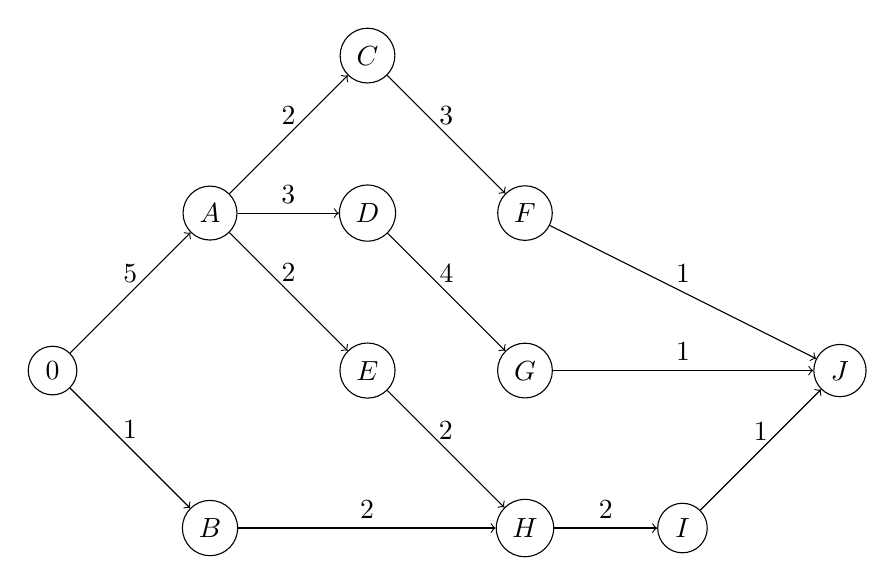
\begin{tikzpicture}[scale=2.0,->]
\node[circle,draw] (0) at (0,1) {$0$};
\node[circle,draw] (A) at (1,2) {$A$};
\node[circle,draw] (B) at (1,0) {$B$};
\node[circle,draw] (C) at (2,3) {$C$};
\node[circle,draw] (D) at (2,2) {$D$};
\node[circle,draw] (E) at (2,1) {$E$};
\node[circle,draw] (F) at (3,2) {$F$};
\node[circle,draw] (G) at (3,1) {$G$};
\node[circle,draw] (H) at (3,0) {$H$};
\node[circle,draw] (I) at (4,0) {$I$};
\node[circle,draw] (J) at (5,1) {$J$};
\path
 (0) edge node[above,midway] {5} (A)
 (0) edge node[above,midway] {1} (B)
 (A) edge node[above,midway] {2} (C)
 (A) edge node[above,midway] {3} (D)
 (A) edge node[above,midway] {2} (E)
 (B) edge node[above,midway] {2} (H)
 (C) edge node[above,midway] {3} (F)
 (D) edge node[above,midway] {4} (G)
 (E) edge node[above,midway] {2} (H)
 (H) edge node[above,midway] {2} (I)
 (I) edge node[above,midway] {1} (J)
 (F) edge node[above,midway] {1} (J)
 (G) edge node[above,midway] {1} (J)
 ;
\end{tikzpicture}
\caption{Graphe du projet commercial}
\label{fig:project}
\end{center}
\end{figure}
\end{example}

\section{Problème de l'arbre partiel minimum}

Considérons un graphe non orienté et connexe.
A chaque arête $\lbrace i,j \rbrace$, nous associons une distance $c_{ij} \geq 0$.
Nous cherchons à construire un arbre partiel (plus petit graphe connexe contenant tous les sommets) dont
la somme des distances soit minimum parmi tous les arbres partiels du graphe.
C'est un exemple simple de problème de conception de réseaux (network design): choisir une
configuration de réseau (sous-ensemble d'arcs) qui optimise un certain critère.

\subsection{Algorithme de Prim (1957)}

Il s'agit à nouveau d'une approche itérative.
L'algorithme est initialisé en choisissant un sommet $i$ (arbitrairement) et en le reliant au sommet $j$ le plus proche.
En d'autres termes, nous ajoutons l'arête $\lbrace i,j \rbrace$.
À chaque itération, nous choisissons le sommet non relié $j$ le plus près d'un des sommets déjà reliés $i$ et nous ajoutons
$\lbrace i,j \rbrace$.
Nous nous arrêtons lorsque tous les sommets ont été reliés.
En cas d'égalité, nous pouvons choisir arbitrairement.
De telles égalités indiquent qu'il pourrait y avoir plusieurs solutions optimales.

\begin{example}
Considérons à nouveau l'exemple~\ref{ex:parc_seervada}.
\begin{enumerate}
 \item 
L'initialisation consiste à choisir le sommet $O$ et à le relier au sommet le plus près: on ajoute $\lbrace O,A \rbrace$.
 \item
Le sommet non relié le plus près de $O$ ou de $A$ est $B$; comme il est plus près de $A$, on ajoute $\lbrace A,B \rbrace$.
 \item
Le sommet non relié le plus près de $O$, de $A$ ou de $B$ est $C$; puisqu'il est plus près de $B$, on ajoute $\lbrace B,C \rbrace$.
 \item
Le sommet non relié le plus près d'un des sommets reliés est $E$; nous ajoutons l'arête $\lbrace B,E \rbrace$,
 \item
Le sommet non relié le plus près d'un des sommets reliés ($E$) est D; nous ajoutons l'arête $\lbrace E,D \rbrace$
 \item
Le sommet non relié le plus près d'un des sommets reliés ($D$) est $T$; nous ajoutons l'arête $\lbrace D,T \rbrace$.
Tous les sommets sont à présent reliés, aussi, nous nous arrêtons.
La valeur optimale correspond à la somme des distances des arêtes ajoutées, soit 14.
\end{enumerate}
L'arbre partiel minimum est représenté en rouge dans la Figure~\ref{fig:prim}.

\begin{figure}[htbp]
\begin{center}
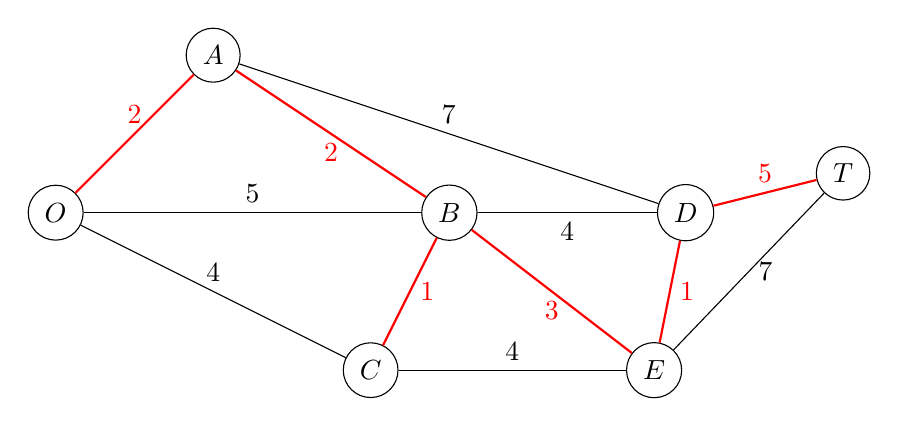
\begin{tikzpicture}
\node[circle,draw] (A) at (2,4) {$A$};
\node[circle,draw] (O) at (0,2) {$O$};
\node[circle,draw] (C) at (4,0) {$C$};
\node[circle,draw] (B) at (5,2) {$B$};
\node[circle,draw] (D) at (8,2) {$D$};
\node[circle,draw] (E) at (7.6,0) {$E$};
\node[circle,draw] (T) at (10,2.5) {$T$};
\path
  (O) edge[color=red,thick] node [above,midway] {2} (A)
  (O) edge node [above,midway] {5} (B)
  (O) edge node [above,midway] {4} (C)
  (A) edge[color=red,thick] node [below,midway] {2} (B)
  (A) edge node [above,midway] {7} (D)
  (B) edge node [below,midway] {4} (D)
  (B) edge[color=red,thick] node [below,midway] {3} (E)
  (E) edge[color=red,thick] node [right,midway] {1} (D)
  (D) edge[color=red,thick] node [above,midway] {5} (T)
  (C) edge[color=red,thick] node [right,midway] {1} (B)
  (E) edge node [right,midway] {7} (T)
  (C) edge node [above,midway] {4} (E)
;
\end{tikzpicture}
\caption{Arbre partiel minimum}
\label{fig:prim}
\end{center}
\end{figure}
\end{example}

\section{Problème du flot maximum}

Considérons un graphe orienté et connexe.
\`A chaque arc $(i,j)$, nous associons une capacité $u_{ij} > 0$.
Il y a deux sommets spéciaux:
\begin{itemize}
 \item 
 source (ou origine) $O$;
 \item
 puits (ou destination) $T$.
\end{itemize}
Tous les autres sont des sommets de transfert.
L'offre en $O$ et la demande en $T$ sont variables.
L'offre en $O$ doit cependant correspondre à la demande en $T$, et indique la valeur du flot entre $O$ et $T$.
Nous cherche à maximiser la valeur du flot entre $O$ et $T$.

Supposons que nous avons déjà affecté un flot sur les arcs.
La {\sl capacité résiduelle} d'un arc $(i,j)$ est comme
\[
  u_{ij} - x_{ij}
\]
Nous définission le {\sl graphe résiduel} comme le graphe non orienté sous-jacent, où, sur chaque arête, nous associons deux valeurs: la capacité résiduelle et le flot déjà affecté.

\begin{example}[Parc Seervada]
 Continuons avec l'exemple~\ref{ex:parc_seervada}, mais en considérant à présent un graphe orienté, comme sur la Figure~\ref{fig:seervada_directed}.
 Supposons qu'en période de grande affluence, nous disposions d'une flotte d'autobus pour faire visiter les différents postes d'observation du parc.
 La réglementation limite le nombre d'autobus pouvant circuler sur chaque tronçon de route.
 Comment faire circuler les autobus dans le parc de façon à maximiser le nombre total d'autobus allant de l'origine ($O$) à la destination ($T$)?

\begin{figure}[htbp]
\begin{center}
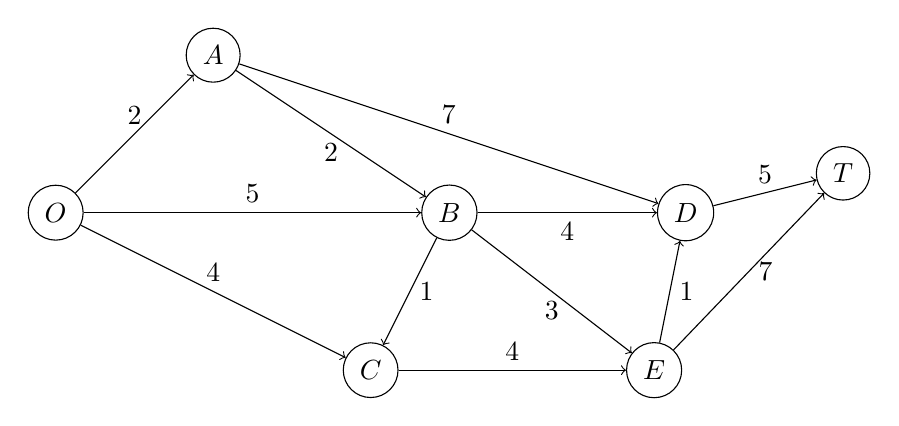
\begin{tikzpicture}[->]
\node[circle,draw] (A) at (2,4) {$A$};
\node[circle,draw] (O) at (0,2) {$O$};
\node[circle,draw] (C) at (4,0) {$C$};
\node[circle,draw] (B) at (5,2) {$B$};
\node[circle,draw] (D) at (8,2) {$D$};
\node[circle,draw] (E) at (7.6,0) {$E$};
\node[circle,draw] (T) at (10,2.5) {$T$};
\path
  (O) edge node [above,midway] {2} (A)
  (O) edge node [above,midway] {5} (B)
  (O) edge node [above,midway] {4} (C)
  (A) edge node [below,midway] {2} (B)
  (A) edge node [above,midway] {7} (D)
  (B) edge node [below,midway] {4} (D)
  (B) edge node [below,midway] {3} (E)
  (E) edge node [right,midway] {1} (D)
  (D) edge node [above,midway] {5} (T)
  (B) edge node [right,midway] {1} (C)
  (E) edge node [right,midway] {7} (T)
  (C) edge node [above,midway] {4} (E)
;
\end{tikzpicture}
\caption{Parc Seervada}
\label{fig:seervada_directed}
\end{center}
\end{figure}

Exemple: nous avons affecté 5 unités de flot sur l'arc (O,B), de capacité 7.
\begin{center}

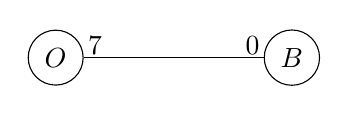
\begin{tikzpicture}
\node[circle,draw] (O) at (0,0) {$O$};
\node[circle,draw] (B) at (3,0) {$B$};
\node at (0.5,0.15) {$7$};
\node at (2.5,0.15) {$0$};
\path
 (O) edge (B)
;
\end{tikzpicture}
 
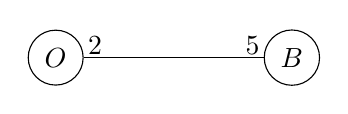
\begin{tikzpicture}
\node[circle,draw] (O) at (0,0) {$O$};
\node[circle,draw] (B) at (3,0) {$B$};
\node at (0.5,0.15) {$2$};
\node at (2.5,0.15) {$5$};
\path
 (O) edge (B)
;
\end{tikzpicture}
\end{center}

Interprétation du graphe résiduel: nous avons affecté 5 unités de flot sur l'arc $(O,B)$.
Si nous traverse $O \rightarrow B$, 2 est la capacité résiduelle et le flot sur $(O, B)$ vaut 5.
Si nous traverse $B \rightarrow O$, la capacité résiduelle est 5 et le flot sur $(B, O)$ vaut 2.

\end{example}

Un chemin d'augmentation est un chemin allant de la source au puits dans le graphe
orienté dérivé du graphe résiduel.
Pour chaque arête $\lbrace i,j \rbrace$, l'arc $(i,j)$ possède une capacité résiduelle $u_{ij} - x_{ij}$, et l'arc $(j,i)$ possède une capacité résiduelle $x_{ij}$.
Chaque arc du chemin possède une capacité résiduelle strictement positive.
La capacité résiduelle d'un chemin d'augmentation est le minimum des capacités résiduelles de tous les arcs du chemin.

\subsection{Algorithme de Ford-Fulkerson}

\begin{algo}{Ford-Fulkerson}
\begin{enumerate}
 \item 
 Initialiser le flot: 0 unité sur chaque arc.
 \item
 Si aucun chemin d'augmentation ne peut être identifié, arrêter: le flot est maximum.
 \item
 Identifier un chemin d'augmentation $P$; soit $c$ sa capacité résiduelle.
 \item
 Sur chaque arc de $P$
 \begin{enumerate}[(a)]
  \item
   augmenter le flot de $c$;
  \item
   diminuer la capacité résiduelle de $c$.
 \end{enumerate}
 \item
 Retourner à l'étape 2.
 \end{enumerate}
\end{algo}

\begin{algo}
Identifier un chemin d'augmentation
\begin{enumerate}
 \item
  Marquer la source $O$ (aucun autre sommet n'est marqué); tous les sommets sont non visités.
 \item
  S'il n'y a aucun sommet marqué non visité, arrêter: il n'existe aucun chemin d'augmentation.
 \item
  Choisir un sommet marqué non visité $i$.
 \item
  Visiter $i$: pour chaque $(i,j)$ de capacité résiduelle strictement positive dans le graphe orienté dérivé du graphe résiduel, marquer $j$.
 \item
  Si $T$ est marqué, arrêter: un chemin d'augmentation a été identifié.
 \item
  Retour à l'étape 2.
\end{enumerate}
\end{algo}

\begin{example}[Parc Seervada: suite]

\mbox{}

\begin{enumerate}
\setcounter{enumi}{-1}
 \item 
Le graphe résiduel initial est représenté sur la Figure~\ref{fig:seervada_residual_initial}.
\begin{figure}[htbp]
\begin{center}
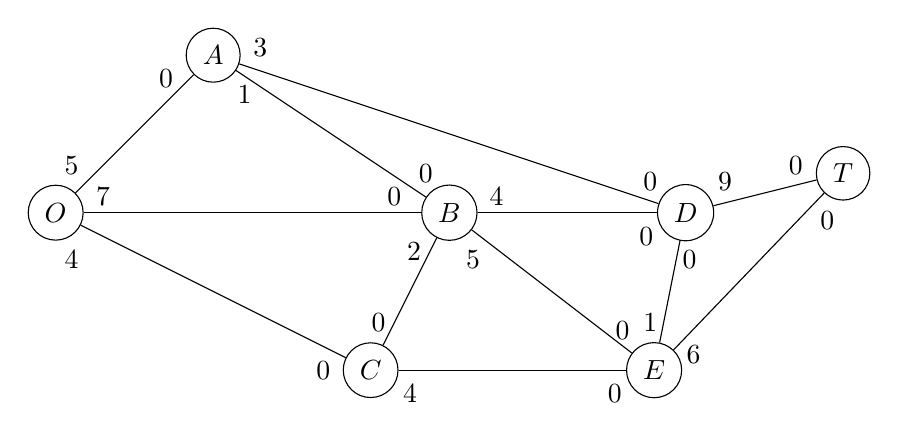
\begin{tikzpicture}
\node[circle,draw] (O) at (0,2) {$O$};
\node at (0.6,2.2) {$7$};
\node at (0.2,2.6) {$5$};
\node at (0.2,1.4) {$4$};
\node[circle,draw] (A) at (2,4) {$A$};
\node at (2.6,4.1) {$3$};
\node at (1.4,3.7) {$0$};
\node at (2.4,3.5) {$1$};
\node[circle,draw] (C) at (4,0) {$C$};
\node at (3.4,0) {$0$};
\node at (4.1,0.6) {$0$};
\node at (4.5,-0.3) {$4$};
\node[circle,draw] (B) at (5,2) {$B$};
\node at (4.3,2.2) {$0$};
\node at (5.6,2.2) {$4$};
\node at (4.7,2.5) {$0$};
\node at (4.55,1.5) {$2$};
\node at (5.3,1.4) {$5$};
\node[circle,draw] (D) at (8,2) {$D$};
\node at (7.5,1.7) {$0$};
\node at (7.55,2.4) {$0$};
\node at (8.05,1.4) {$0$};
\node at (8.5,2.4) {$9$};
\node[circle,draw] (E) at (7.6,0) {$E$};
\node at (7.1,-0.3) {$0$};
\node at (7.2,0.5) {$0$};
\node at (8.1,0.2) {$6$};
\node at (7.55,0.6) {$1$};
\node[circle,draw] (T) at (10,2.5) {$T$};
\node at (9.4,2.6) {$0$};
\node at (9.8,1.9) {$0$};
\path
  (O) edge (A)
  (O) edge (B)
  (O) edge (C)
  (A) edge (B)
  (A) edge (D)
  (B) edge (D)
  (B) edge (E)
  (E) edge (D)
  (D) edge (T)
  (B) edge (C)
  (E) edge (T)
  (C) edge (E)
;
\end{tikzpicture}
\caption{Parc Seervada: initialisation.}
\label{fig:seervada_residual_initial}
\end{center}
\end{figure}
\item
Nous pouvons identifier le chemin d'augmentation $O \rightarrow B \rightarrow E \rightarrow T$.
La capacité résiduelle vaut alors $\min \lbrace 7,5,6 \rbrace = 5$.
En suivant l'algorithme, nous augmentons le flot et diminuons la capacité résiduelle de 5 unités sur tous les arcs de $O \rightarrow B \rightarrow E \rightarrow T$, ce qui conduit au graphe de la Figure~\ref{fig:seervada_residual_1}.
\begin{figure}[htbp]
\begin{center}
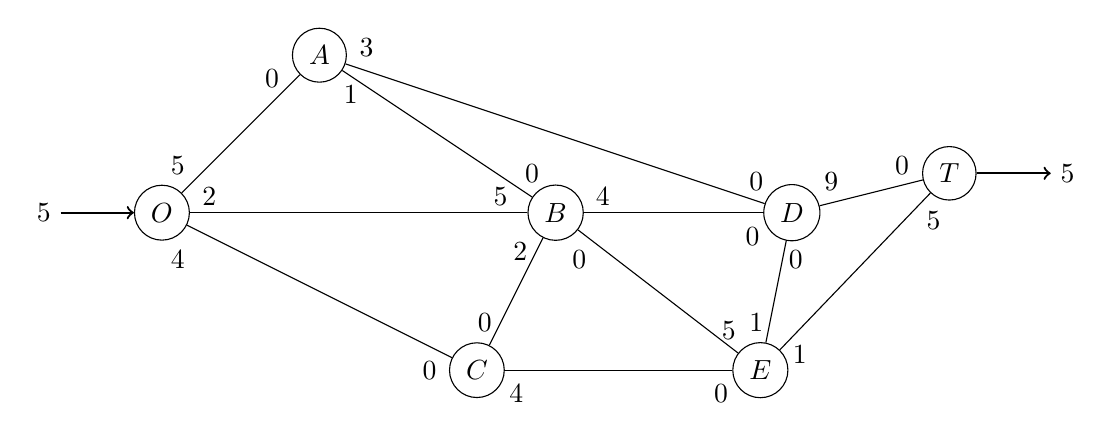
\begin{tikzpicture}
\node (O1) at (-1.5,2) {$5$};
\node (T1) at (11.5,2.5) {$5$};
\node[circle,draw] (O) at (0,2) {$O$};
\node at (0.2,2.6) {$5$};
\node at (0.6,2.2) {$2$};
\node at (0.2,1.4) {$4$};
\node[circle,draw] (A) at (2,4) {$A$};
\node at (1.4,3.7) {$0$};
\node at (2.6,4.1) {$3$};
\node at (2.4,3.5) {$1$};
\node[circle,draw] (B) at (5,2) {$B$};
\node at (4.3,2.2) {$5$};
\node at (4.7,2.5) {$0$};
\node at (5.6,2.2) {$4$};
\node at (5.3,1.4) {$0$};
\node at (4.55,1.5) {$2$};
\node[circle,draw] (C) at (4,0) {$C$};
\node at (3.4,0) {$0$};
\node at (4.1,0.6) {$0$};
\node at (4.5,-0.3) {$4$};
\node[circle,draw] (D) at (8,2) {$D$};
\node at (7.5,1.7) {$0$};
\node at (7.55,2.4) {$0$};
\node at (8.5,2.4) {$9$};
\node at (8.05,1.4) {$0$};
\node[circle,draw] (E) at (7.6,0) {$E$};
\node at (7.1,-0.3) {$0$};
\node at (7.2,0.5) {$5$};
\node at (7.55,0.6) {$1$};
\node at (8.1,0.2) {$1$};
\node[circle,draw] (T) at (10,2.5) {$T$};
\node at (9.4,2.6) {$0$};
\node at (9.8,1.9) {$5$};
\path
  (O) edge (A)
  (O) edge (B)
  (O) edge (C)
  (A) edge (B)
  (A) edge (D)
  (B) edge (D)
  (B) edge (E)
  (E) edge (D)
  (D) edge (T)
  (B) edge (C)
  (E) edge (T)
  (C) edge (E)
  (O1) edge [->, thick] (O)
  (T) edge [->, thick] (T1)
;
\end{tikzpicture}
\caption{Parc Seervada: itération 1.}
\label{fig:seervada_residual_1}
\end{center}
\end{figure}
\item
Nous pouvons à présent identifier le chemin d'augmentation $O \rightarrow A \rightarrow D \rightarrow T$, qui donne une capacité résiduelle de $\min \lbrace 5,3,9 \rbrace = 3$.
Nous augmentons le flot et diminuons la capacité résiduelle de 3 unités sur tous les arcs de $O \rightarrow A \rightarrow D \rightarrow T$,
comme représenté sur la Figure~\ref{fig:seervada_residual_2}.
\begin{figure}[htbp]
\begin{center}
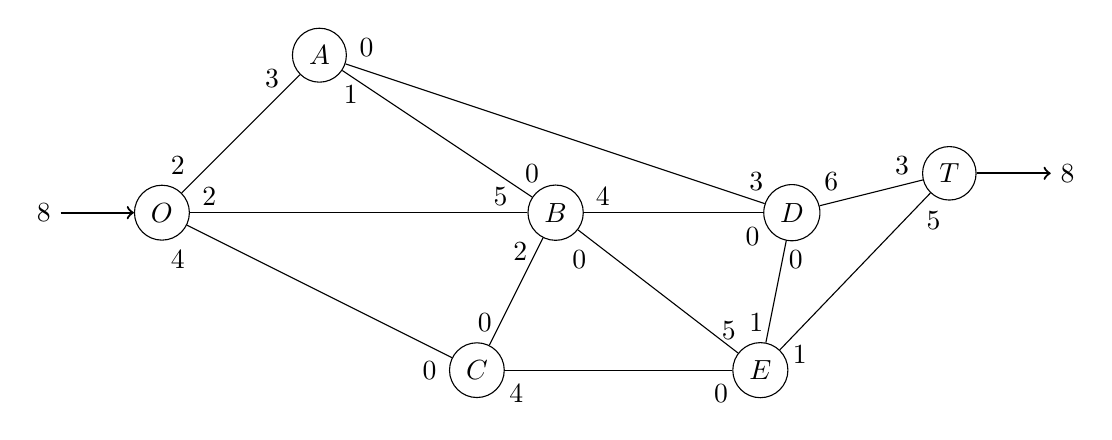
\begin{tikzpicture}
\node (O1) at (-1.5,2) {$8$};
\node (T1) at (11.5,2.5) {$8$};
\node[circle,draw] (O) at (0,2) {$O$};
\node at (0.2,2.6) {$2$};
\node at (0.6,2.2) {$2$};
\node at (0.2,1.4) {$4$};
\node[circle,draw] (A) at (2,4) {$A$};
\node at (1.4,3.7) {$3$};
\node at (2.6,4.1) {$0$};
\node at (2.4,3.5) {$1$};
\node[circle,draw] (B) at (5,2) {$B$};
\node at (4.3,2.2) {$5$};
\node at (4.7,2.5) {$0$};
\node at (5.6,2.2) {$4$};
\node at (5.3,1.4) {$0$};
\node at (4.55,1.5) {$2$};
\node[circle,draw] (C) at (4,0) {$C$};
\node at (3.4,0) {$0$};
\node at (4.1,0.6) {$0$};
\node at (4.5,-0.3) {$4$};
\node[circle,draw] (D) at (8,2) {$D$};
\node at (7.5,1.7) {$0$};
\node at (7.55,2.4) {$3$};
\node at (8.5,2.4) {$6$};
\node at (8.05,1.4) {$0$};
\node[circle,draw] (E) at (7.6,0) {$E$};
\node at (7.1,-0.3) {$0$};
\node at (7.2,0.5) {$5$};
\node at (7.55,0.6) {$1$};
\node at (8.1,0.2) {$1$};
\node[circle,draw] (T) at (10,2.5) {$T$};
\node at (9.4,2.6) {$3$};
\node at (9.8,1.9) {$5$};
\path
  (O) edge (A)
  (O) edge (B)
  (O) edge (C)
  (A) edge (B)
  (A) edge (D)
  (B) edge (D)
  (B) edge (E)
  (E) edge (D)
  (D) edge (T)
  (B) edge (C)
  (E) edge (T)
  (C) edge (E)
  (O1) edge [->, thick] (O)
  (T) edge [->, thick] (T1)
;
\end{tikzpicture}
\caption{Parc Seervada: itération 2.}
\label{fig:seervada_residual_2}
\end{center}
\end{figure}
\item
Nous avons le chemin d'augmentation $O \rightarrow A \rightarrow B \rightarrow D \rightarrow T$, et la capacité résiduelle $\min \lbrace 2,1,4,6 \rbrace = 1$.
Augmentons le flot et diminuons la capacité résiduelle de 1 unité sur tous les arcs de $O \rightarrow A \rightarrow B \rightarrow D \rightarrow T$, pour obtenir la Figure~\ref{fig:seervada_residual_3}.
\begin{figure}[htbp]
\begin{center}
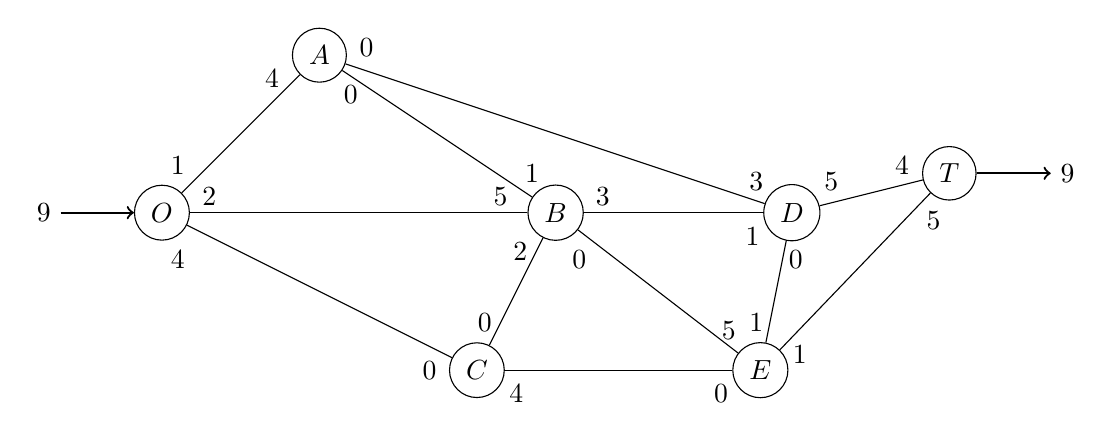
\begin{tikzpicture}
\node (O1) at (-1.5,2) {$9$};
\node (T1) at (11.5,2.5) {$9$};
\node[circle,draw] (O) at (0,2) {$O$};
\node at (0.2,2.6) {$1$};
\node at (0.6,2.2) {$2$};
\node at (0.2,1.4) {$4$};
\node[circle,draw] (A) at (2,4) {$A$};
\node at (1.4,3.7) {$4$};
\node at (2.6,4.1) {$0$};
\node at (2.4,3.5) {$0$};
\node[circle,draw] (B) at (5,2) {$B$};
\node at (4.3,2.2) {$5$};
\node at (4.7,2.5) {$1$};
\node at (5.6,2.2) {$3$};
\node at (5.3,1.4) {$0$};
\node at (4.55,1.5) {$2$};
\node[circle,draw] (C) at (4,0) {$C$};
\node at (3.4,0) {$0$};
\node at (4.1,0.6) {$0$};
\node at (4.5,-0.3) {$4$};
\node[circle,draw] (D) at (8,2) {$D$};
\node at (7.5,1.7) {$1$};
\node at (7.55,2.4) {$3$};
\node at (8.5,2.4) {$5$};
\node at (8.05,1.4) {$0$};
\node[circle,draw] (E) at (7.6,0) {$E$};
\node at (7.1,-0.3) {$0$};
\node at (7.2,0.5) {$5$};
\node at (7.55,0.6) {$1$};
\node at (8.1,0.2) {$1$};
\node[circle,draw] (T) at (10,2.5) {$T$};
\node at (9.4,2.6) {$4$};
\node at (9.8,1.9) {$5$};
\path
  (O) edge (A)
  (O) edge (B)
  (O) edge (C)
  (A) edge (B)
  (A) edge (D)
  (B) edge (D)
  (B) edge (E)
  (E) edge (D)
  (D) edge (T)
  (B) edge (C)
  (E) edge (T)
  (C) edge (E)
  (O1) edge [->, thick] (O)
  (T) edge [->, thick] (T1)
;
\end{tikzpicture}
\caption{Parc Seervada: itération 3.}
\label{fig:seervada_residual_3}
\end{center}
\end{figure}
\item
Identifions le chemin d'augmentation $O \rightarrow B \rightarrow D \rightarrow T$, ce qui donne comme apacité résiduelle $\min \lbrace 2,3,5 \rbrace = 2$.
Nous augmentons le flot et diminuer la capacité résiduelle de 2 unités sur tous les arcs de $O \rightarrow B \rightarrow D \rightarrow T$, ce qui conduite à la Figure~\ref{fig:seervada_residual_4}..
\begin{figure}[htbp]
\begin{center}
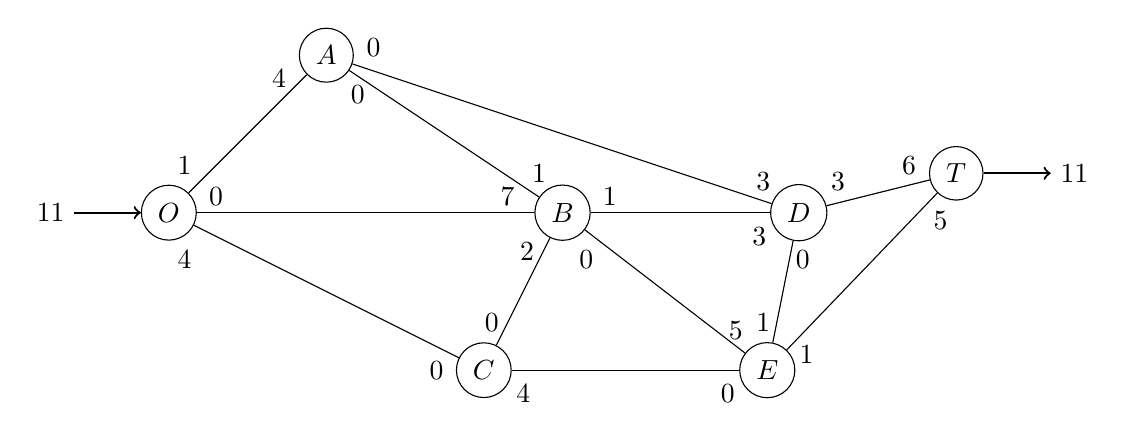
\begin{tikzpicture}
\node (O1) at (-1.5,2) {$11$};
\node (T1) at (11.5,2.5) {$11$};
\node[circle,draw] (O) at (0,2) {$O$};
\node at (0.2,2.6) {$1$};
\node at (0.6,2.2) {$0$};
\node at (0.2,1.4) {$4$};
\node[circle,draw] (A) at (2,4) {$A$};
\node at (1.4,3.7) {$4$};
\node at (2.6,4.1) {$0$};
\node at (2.4,3.5) {$0$};
\node[circle,draw] (B) at (5,2) {$B$};
\node at (4.3,2.2) {$7$};
\node at (4.7,2.5) {$1$};
\node at (5.6,2.2) {$1$};
\node at (5.3,1.4) {$0$};
\node at (4.55,1.5) {$2$};
\node[circle,draw] (C) at (4,0) {$C$};
\node at (3.4,0) {$0$};
\node at (4.1,0.6) {$0$};
\node at (4.5,-0.3) {$4$};
\node[circle,draw] (D) at (8,2) {$D$};
\node at (7.5,1.7) {$3$};
\node at (7.55,2.4) {$3$};
\node at (8.5,2.4) {$3$};
\node at (8.05,1.4) {$0$};
\node[circle,draw] (E) at (7.6,0) {$E$};
\node at (7.1,-0.3) {$0$};
\node at (7.2,0.5) {$5$};
\node at (7.55,0.6) {$1$};
\node at (8.1,0.2) {$1$};
\node[circle,draw] (T) at (10,2.5) {$T$};
\node at (9.4,2.6) {$6$};
\node at (9.8,1.9) {$5$};
\path
  (O) edge (A)
  (O) edge (B)
  (O) edge (C)
  (A) edge (B)
  (A) edge (D)
  (B) edge (D)
  (B) edge (E)
  (E) edge (D)
  (D) edge (T)
  (B) edge (C)
  (E) edge (T)
  (C) edge (E)
  (O1) edge [->, thick] (O)
  (T) edge [->, thick] (T1)
;
\end{tikzpicture}
\caption{Parc Seervada: itération 4.}
\label{fig:seervada_residual_4}
\end{center}
\end{figure}
\item
Prenons le chemin d'augmentation $O \rightarrow C \rightarrow E \rightarrow D \rightarrow T$, avec comme capacité résiduelle $\min \lbrace 4,4,1,3 \rbrace = 1$.
Ceci nous conduit à augmenter le flot et diminuer la capacité résiduelle de 1 unité sur tous les arcs de $O \rightarrow C \rightarrow E \rightarrow D \rightarrow T$.
Nous obtenons ainsi le graphe de la Figure~\ref{fig:seervada_residual_5}.
\begin{figure}[htbp]
\begin{center}
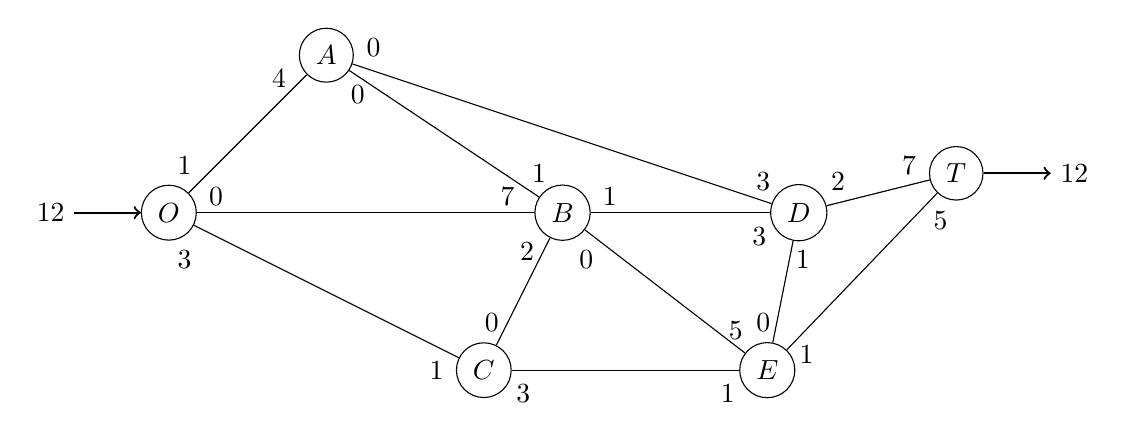
\begin{tikzpicture}
\node (O1) at (-1.5,2) {$12$};
\node (T1) at (11.5,2.5) {$12$};
\node[circle,draw] (O) at (0,2) {$O$};
\node at (0.2,2.6) {$1$};
\node at (0.6,2.2) {$0$};
\node at (0.2,1.4) {$3$};
\node[circle,draw] (A) at (2,4) {$A$};
\node at (1.4,3.7) {$4$};
\node at (2.6,4.1) {$0$};
\node at (2.4,3.5) {$0$};
\node[circle,draw] (B) at (5,2) {$B$};
\node at (4.3,2.2) {$7$};
\node at (4.7,2.5) {$1$};
\node at (5.6,2.2) {$1$};
\node at (5.3,1.4) {$0$};
\node at (4.55,1.5) {$2$};
\node[circle,draw] (C) at (4,0) {$C$};
\node at (3.4,0) {$1$};
\node at (4.1,0.6) {$0$};
\node at (4.5,-0.3) {$3$};
\node[circle,draw] (D) at (8,2) {$D$};
\node at (7.5,1.7) {$3$};
\node at (7.55,2.4) {$3$};
\node at (8.5,2.4) {$2$};
\node at (8.05,1.4) {$1$};
\node[circle,draw] (E) at (7.6,0) {$E$};
\node at (7.1,-0.3) {$1$};
\node at (7.2,0.5) {$5$};
\node at (7.55,0.6) {$0$};
\node at (8.1,0.2) {$1$};
\node[circle,draw] (T) at (10,2.5) {$T$};
\node at (9.4,2.6) {$7$};
\node at (9.8,1.9) {$5$};
\path
  (O) edge (A)
  (O) edge (B)
  (O) edge (C)
  (A) edge (B)
  (A) edge (D)
  (B) edge (D)
  (B) edge (E)
  (E) edge (D)
  (D) edge (T)
  (B) edge (C)
  (E) edge (T)
  (C) edge (E)
  (O1) edge [->, thick] (O)
  (T) edge [->, thick] (T1)
;
\end{tikzpicture}
\caption{Parc Seervada: itération 5.}
\label{fig:seervada_residual_5}
\end{center}
\end{figure}
\item
Nous pouvons choisir le chemin d'augmentation $O \rightarrow C \rightarrow E \rightarrow T$.
La capacité résiduelle est $\min \lbrace 3,3,1 \rbrace = 1$.
En augmentant le flot et en diminuant la capacité résiduelle de 1 unité sur tous les arcs de $O \rightarrow C \rightarrow E \rightarrow T$, nous obtenons la Figure~\ref{fig:seervada_residual_6}.
\begin{figure}[htbp]
\begin{center}
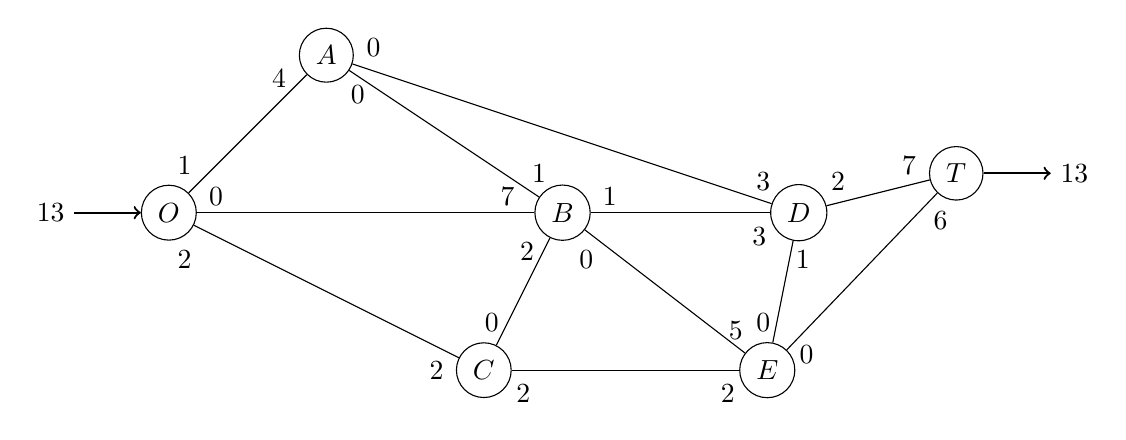
\begin{tikzpicture}
\node (O1) at (-1.5,2) {$13$};
\node (T1) at (11.5,2.5) {$13$};
\node[circle,draw] (O) at (0,2) {$O$};
\node at (0.2,2.6) {$1$};
\node at (0.6,2.2) {$0$};
\node at (0.2,1.4) {$2$};
\node[circle,draw] (A) at (2,4) {$A$};
\node at (1.4,3.7) {$4$};
\node at (2.6,4.1) {$0$};
\node at (2.4,3.5) {$0$};
\node[circle,draw] (B) at (5,2) {$B$};
\node at (4.3,2.2) {$7$};
\node at (4.7,2.5) {$1$};
\node at (5.6,2.2) {$1$};
\node at (5.3,1.4) {$0$};
\node at (4.55,1.5) {$2$};
\node[circle,draw] (C) at (4,0) {$C$};
\node at (3.4,0) {$2$};
\node at (4.1,0.6) {$0$};
\node at (4.5,-0.3) {$2$};
\node[circle,draw] (D) at (8,2) {$D$};
\node at (7.5,1.7) {$3$};
\node at (7.55,2.4) {$3$};
\node at (8.5,2.4) {$2$};
\node at (8.05,1.4) {$1$};
\node[circle,draw] (E) at (7.6,0) {$E$};
\node at (7.1,-0.3) {$2$};
\node at (7.2,0.5) {$5$};
\node at (7.55,0.6) {$0$};
\node at (8.1,0.2) {$0$};
\node[circle,draw] (T) at (10,2.5) {$T$};
\node at (9.4,2.6) {$7$};
\node at (9.8,1.9) {$6$};
\path
  (O) edge (A)
  (O) edge (B)
  (O) edge (C)
  (A) edge (B)
  (A) edge (D)
  (B) edge (D)
  (B) edge (E)
  (E) edge (D)
  (D) edge (T)
  (B) edge (C)
  (E) edge (T)
  (C) edge (E)
  (O1) edge [->, thick] (O)
  (T) edge [->, thick] (T1)
;
\end{tikzpicture}
\caption{Parc Seervada: itération 6.}
\label{fig:seervada_residual_6}
\end{center}
\end{figure}
\item
Considérons le chemin d'augmentation: $O \rightarrow C \rightarrow E \rightarrow B \rightarrow D \rightarrow T$, de capacité résiduelle $\min \lbrace 2,2,5,1,2 \rbrace = 1$.
Par conséquent, nous augmenter le flot et diminuons la capacité résiduelle de 1 unité sur tous les arcs de $O \rightarrow C \rightarrow E \rightarrow B \rightarrow D \rightarrow T$,
ce qui donne la Figure~\ref{fig:seervada_residual_7}.
\begin{figure}[htbp]
\begin{center}
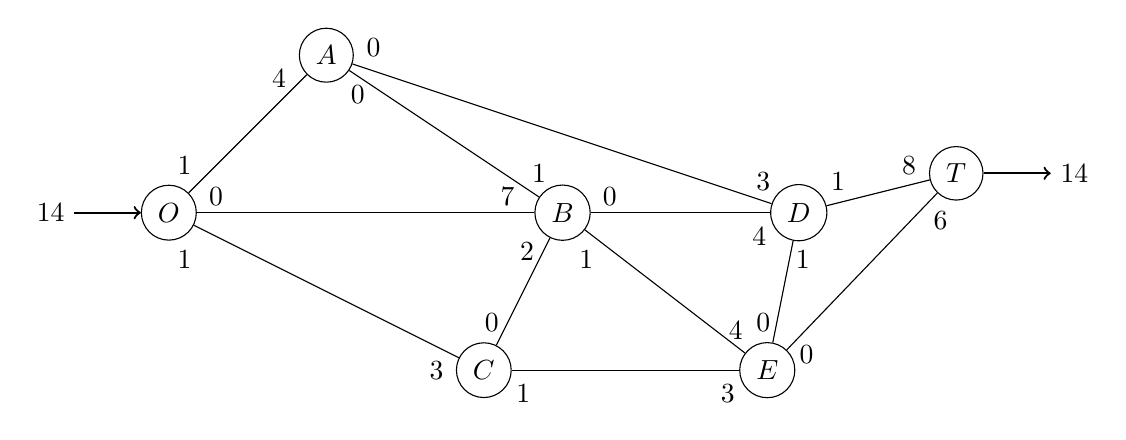
\begin{tikzpicture}
\node (O1) at (-1.5,2) {$14$};
\node (T1) at (11.5,2.5) {$14$};
\node[circle,draw] (O) at (0,2) {$O$};
\node at (0.2,2.6) {$1$};
\node at (0.6,2.2) {$0$};
\node at (0.2,1.4) {$1$};
\node[circle,draw] (A) at (2,4) {$A$};
\node at (1.4,3.7) {$4$};
\node at (2.6,4.1) {$0$};
\node at (2.4,3.5) {$0$};
\node[circle,draw] (B) at (5,2) {$B$};
\node at (4.3,2.2) {$7$};
\node at (4.7,2.5) {$1$};
\node at (5.6,2.2) {$0$};
\node at (5.3,1.4) {$1$};
\node at (4.55,1.5) {$2$};
\node[circle,draw] (C) at (4,0) {$C$};
\node at (3.4,0) {$3$};
\node at (4.1,0.6) {$0$};
\node at (4.5,-0.3) {$1$};
\node[circle,draw] (D) at (8,2) {$D$};
\node at (7.5,1.7) {$4$};
\node at (7.55,2.4) {$3$};
\node at (8.5,2.4) {$1$};
\node at (8.05,1.4) {$1$};
\node[circle,draw] (E) at (7.6,0) {$E$};
\node at (7.1,-0.3) {$3$};
\node at (7.2,0.5) {$4$};
\node at (7.55,0.6) {$0$};
\node at (8.1,0.2) {$0$};
\node[circle,draw] (T) at (10,2.5) {$T$};
\node at (9.4,2.6) {$8$};
\node at (9.8,1.9) {$6$};
\path
  (O) edge (A)
  (O) edge (B)
  (O) edge (C)
  (A) edge (B)
  (A) edge (D)
  (B) edge (D)
  (B) edge (E)
  (E) edge (D)
  (D) edge (T)
  (B) edge (C)
  (E) edge (T)
  (C) edge (E)
  (O1) edge [->, thick] (O)
  (T) edge [->, thick] (T1)
;
\end{tikzpicture}
\caption{Parc Seervada: itération 7.}
\label{fig:seervada_residual_7}
\end{center}
\end{figure}
\item
Il n'y a plus aucun chemin d'augmentation possible; nous avons atteint le flot maximum, lequel est réparti comme représenté sur la Figure~\ref{fig:seervada_fin}.
\begin{figure}[htbp]
\begin{center}
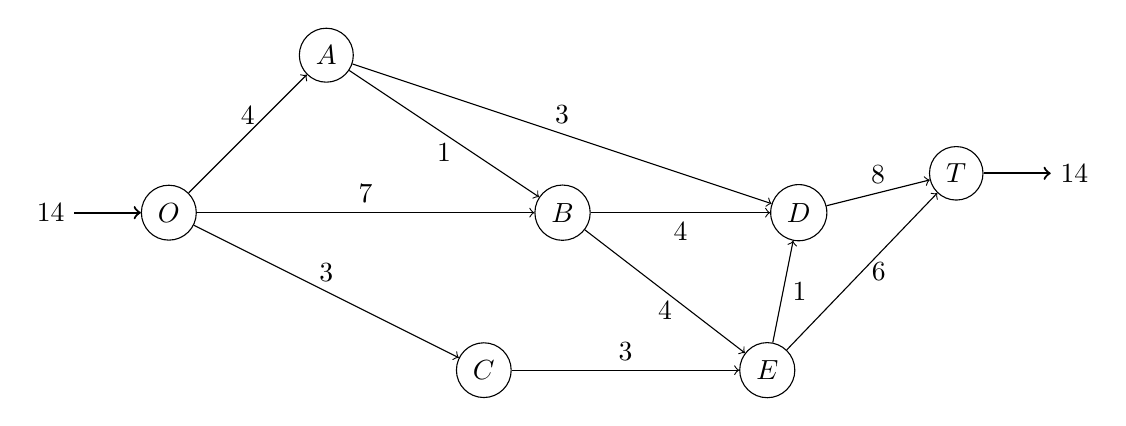
\begin{tikzpicture}[->]
\node (O1) at (-1.5,2) {$14$};
\node (T1) at (11.5,2.5) {$14$};
\node[circle,draw] (O) at (0,2) {$O$};
\node[circle,draw] (A) at (2,4) {$A$};
\node[circle,draw] (C) at (4,0) {$C$};
\node[circle,draw] (B) at (5,2) {$B$};
\node[circle,draw] (D) at (8,2) {$D$};
\node[circle,draw] (E) at (7.6,0) {$E$};
\node[circle,draw] (T) at (10,2.5) {$T$};
\path
  (O) edge node [above,midway] {4} (A)
  (O) edge node [above,midway] {7} (B)
  (O) edge node [above,midway] {3} (C)
  (A) edge node [below,midway] {1} (B)
  (A) edge node [above,midway] {3} (D)
  (B) edge node [below,midway] {4} (D)
  (B) edge node [below,midway] {4} (E)
  (C) edge node [above,midway] {3} (E)
  (D) edge node [above,midway] {8} (T)
  (E) edge node [right,midway] {1} (D)
  (E) edge node [right,midway] {6} (T)
  (O1) edge [->, thick] (O)
  (T) edge [->, thick] (T1)
;
\end{tikzpicture}
\caption{Parc Seervada: fin.}
\label{fig:seervada_fin}
\end{center}
\end{figure}
\end{enumerate}
\end{example}

\subsection{Flot maximum - Coupe minimum}

Supposons que nous partitionnions l'ensemble des sommets en deux sous-ensembles $X$, $Y$.
Une {\sl coupe} est un sous-ensemble d'arcs allant d'un sommet de $X$ vers un sommet de $Y$.
La capacité d'une coupe est la somme des capacités des arcs de la coupe.
Une coupe minimum est une coupe dont la capacité est minimum parmi toutes les coupes possibles.
Le théorème flot max--coupe min dit que la valeur du flot maximum est égale à la capacité d'une coupe minimum.
Les sommets marqués lors de la dernière itération de
l'algorithme de Ford-Fulkerson définissent la coupe minimum, comme illustré sur la Figure~\ref{fig:seervada_coupe} pour l'exemple du parc Seervada.

\begin{figure}[htbp]
\begin{center}
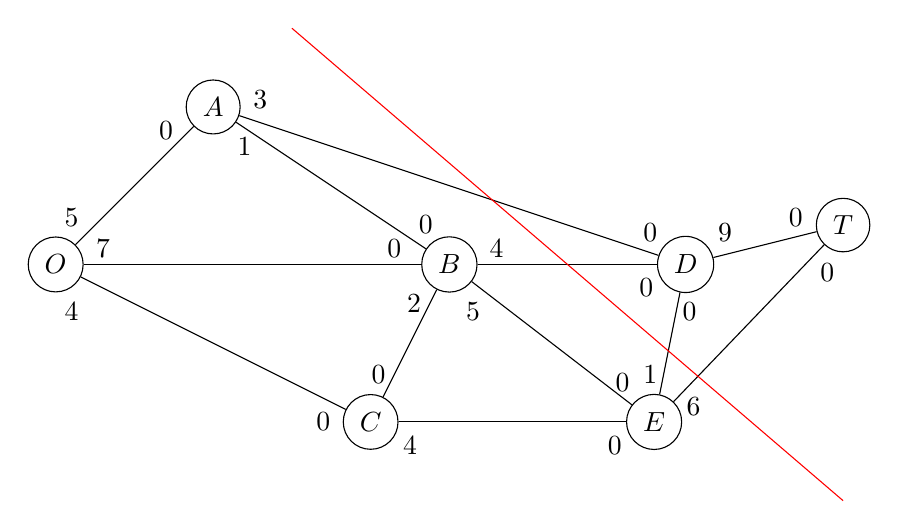
\begin{tikzpicture}
\node[circle,draw] (O) at (0,2) {$O$};
\node at (0.6,2.2) {$7$};
\node at (0.2,2.6) {$5$};
\node at (0.2,1.4) {$4$};
\node[circle,draw] (A) at (2,4) {$A$};
\node at (2.6,4.1) {$3$};
\node at (1.4,3.7) {$0$};
\node at (2.4,3.5) {$1$};
\node[circle,draw] (C) at (4,0) {$C$};
\node at (3.4,0) {$0$};
\node at (4.1,0.6) {$0$};
\node at (4.5,-0.3) {$4$};
\node[circle,draw] (B) at (5,2) {$B$};
\node at (4.3,2.2) {$0$};
\node at (5.6,2.2) {$4$};
\node at (4.7,2.5) {$0$};
\node at (4.55,1.5) {$2$};
\node at (5.3,1.4) {$5$};
\node[circle,draw] (D) at (8,2) {$D$};
\node at (7.5,1.7) {$0$};
\node at (7.55,2.4) {$0$};
\node at (8.05,1.4) {$0$};
\node at (8.5,2.4) {$9$};
\node[circle,draw] (E) at (7.6,0) {$E$};
\node at (7.1,-0.3) {$0$};
\node at (7.2,0.5) {$0$};
\node at (8.1,0.2) {$6$};
\node at (7.55,0.6) {$1$};
\node[circle,draw] (T) at (10,2.5) {$T$};
\node at (9.4,2.6) {$0$};
\node at (9.8,1.9) {$0$};
\path
  (O) edge (A)
  (O) edge (B)
  (O) edge (C)
  (A) edge (B)
  (A) edge (D)
  (B) edge (D)
  (B) edge (E)
  (E) edge (D)
  (D) edge (T)
  (B) edge (C)
  (E) edge (T)
  (C) edge (E)
;
\draw[color=red] (3,5) -- (10,-1); 
\end{tikzpicture}
\caption{Parc Seervada: coupe minimum.}
\label{fig:seervada_coupe}
\end{center}
\end{figure}

\section{Problème de flot minimum}

Plutôt que de maximiser le flot sur le réseau, nous pourrions chercher à trouver la façon la plus économique d'envoyer un certain flot à travers un réseau.
Considérons un réseau de flot $G(N,A)$, avec une source $s \in N$ et un puits $t \in N$. On veut envoyer le flux $d$ de $s$ à $t$.
Soient $\ell(i,j)$ le coût unitaire sur l'arête $\lbrace i, i \rbrace$, et $f(i,j)$ le flot $\lbrace i, j \rbrace$.
Nous avons le problème linéaire
\begin{align*}
\min\ &\sum_{i,j \in N} \ell(i,j)f(i,j), \\
\sc{}\ & f(i,j) \leq c_{ij}, \\
& f(i,j) = -f(j,i), \\
& \sum_{k \in N} f(i,k) = 0,\ \forall k \ne s,t,\\
& \sum_{k \in N} f(s,k) = \sum_{k \in N} f(k,t) = d.\\
\end{align*}

\begin{small}
\section{Notes}

Ce chapitre se base partiellement sur les notes de cours de Bernard Gendron, 2007.
La section sur les plus cours chemins repose également sur du matériel de cours mis en ligne par Otfried Cheong.

\end{small}
